%! alt Square ABCD of side s, with P on AB, Q on BC, R on CD and S on DA, drawn for s = 24. The diagonals of quadrilateral PQRS are PR = 25 and QS = 31. Its area is half the size of the cross product of these two diagonals.
%! after_paragraph 2
%! scale 1/4
% The shared preamble of every Kyuclid figure. pipeline/figures turns these colours into theme-aware paint,
% and refuses any other colour, so draw only with them:
%   figink (lines and labels), figaux (construction lines), figaccent (the object the argument turns on),
%   figtint and figaccenttint (light fills).
\documentclass[border=1.5pt]{standalone}
\usepackage{tkz-euclide}
\definecolor{figink}{RGB}{0,0,0}
\definecolor{figaux}{RGB}{85,85,85}
\definecolor{figaccent}{RGB}{192,57,43}
\definecolor{figtint}{RGB}{221,221,221}
\definecolor{figaccenttint}{RGB}{245,213,208}
% tkz-euclide's defaults draw circles, compasses and marks in 50% grey and fill points with a tint.
\makeatletter
\def\tkz@otherlinecolor{figink}
\def\tkz@euc@circlecolor{figink}
\def\tkz@euc@compasscolor{figink}
\def\tkz@euc@mkcolor{figink}
\def\tkz@mk@fill{figink}
\def\tkz@euc@pointfillcolor{figink}
\makeatother
\tkzSetUpLine[color=figink,line width=.7pt]
\tkzSetUpArc[color=figink,line width=.7pt]
\tkzSetUpCompass[color=figink,line width=.5pt]
\tkzSetUpPoint[color=figink,fill=figink,size=3.1pt]
\tikzset{
  every picture/.style={line cap=round,line join=round,color=figink},
  circle style/.append style={color=figink,line width=.7pt},
  aux/.style={color=figaux,line width=.45pt,dash pattern=on 2.6pt off 2pt},
  key/.style={color=figaccent,line width=1pt},
  mk/.style={color=figink,line width=.5pt},
  lbl/.style={color=figink,inner sep=2.2pt},
  len/.style={color=figink,inner sep=1.5pt,font=\small},
}

\begin{document}
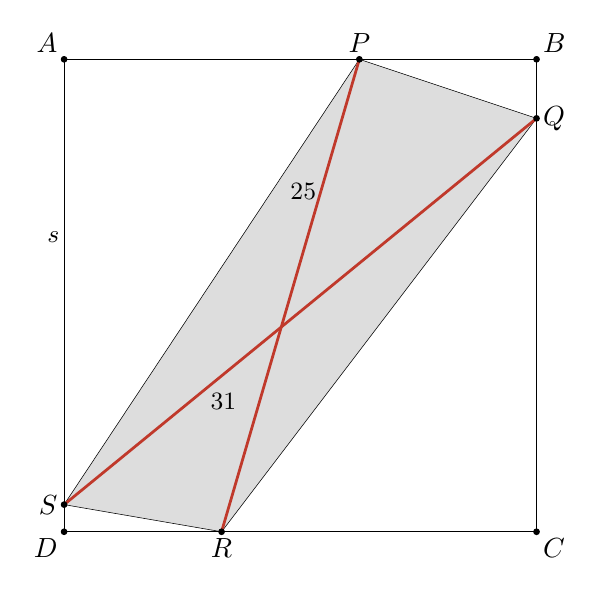
\begin{tikzpicture}
\tkzDefPoint(0.0,6.0000000){A} %! A = (0, 24)
\tkzDefPoint(6.0000000,6.0000000){B} %! B = (24, 24)
\tkzDefPoint(6.0000000,0.0){C} %! C = (24, 0)
\tkzDefPoint(0.0,0.0){D} %! D = (0, 0)
\tkzDefPoint(3.7500000,6.0000000){P} %! P = (15, 24)
\tkzDefPoint(2.0000000,0.0){R} %! R = (8, 0)
\tkzDefPoint(6.0000000,5.2500000){Q} %! Q = (24, 21)
\tkzDefPoint(0.0,0.34464578){S} %! S = (0, 21 - sqrt(385))
%! fact dist(P, R) == 25
%! fact dist(Q, S) == 31
%! fact on_segment(P, A, B)
%! fact on_segment(Q, B, C)
%! fact on_segment(R, C, D)
%! fact on_segment(S, D, A)
%! fact perp(A, B, B, C)
%! fact equal(dist(A, B), dist(B, C))
\tkzFillPolygon[color=figtint](P,Q,R,S)
\tkzDrawPolygon(A,B,C,D)
\tkzDrawPolygon(P,Q,R,S)
\tkzDrawSegments[key](P,R Q,S)
\tkzDrawPoints(A,B,C,D,P,Q,R,S)
\tkzLabelPoint[above left,lbl](A){$A$}
\tkzLabelPoint[above right,lbl](B){$B$}
\tkzLabelPoint[below right,lbl](C){$C$}
\tkzLabelPoint[below left,lbl](D){$D$}
\tkzLabelPoint[above,lbl](P){$P$}
\tkzLabelPoint[right,lbl](Q){$Q$}
\tkzLabelPoint[below,lbl](R){$R$}
\tkzLabelPoint[left,lbl](S){$S$}
\tkzLabelSegment[left,pos=.72,len](R,P){$25$}
\tkzLabelSegment[below right,pos=.3,len](S,Q){$31$}
\tkzLabelSegment[left,pos=.6,len](S,A){$s$}
\end{tikzpicture}
\end{document}
